\chapter{Neural Networks}
\label{chap:nn}

\begin{description}
  \item[Motivation.] Obtain a glimpse of how deep learning can enter modern
  econometrics.
  \item[Neural networks.] Build a flexible global approximation from simple
  layers.
  \item[Conditional expectations.] Connect squared-error training to nuisance
  functions used in causal inference.
  \item[Application.] Introduce DeepIV and large-scale heterogeneous position
  effects in sponsored search.
\end{description}

\section{Neural networks as function approximators}

Neural networks are the basic building blocks of deep learning.  They are used
for many tasks, but our focus is function approximation.  CATE and CLATE are
functions of covariates, while ATE, ATT, and LATE estimators often depend on
conditional means or probabilities.  Earlier chapters used regression trees
and forests to estimate such functions.  Neural networks provide a global,
smooth alternative.

Consider $x=(x_1,x_2,x_3)'$ and an unknown real-valued function $h(x)$.  A
one-hidden-layer network constructs a parameterized approximation
$h_\theta(x)$, as illustrated in Figure~\ref{fig:nn-schematic}.

\begin{figure}[tbp]
  \centering
  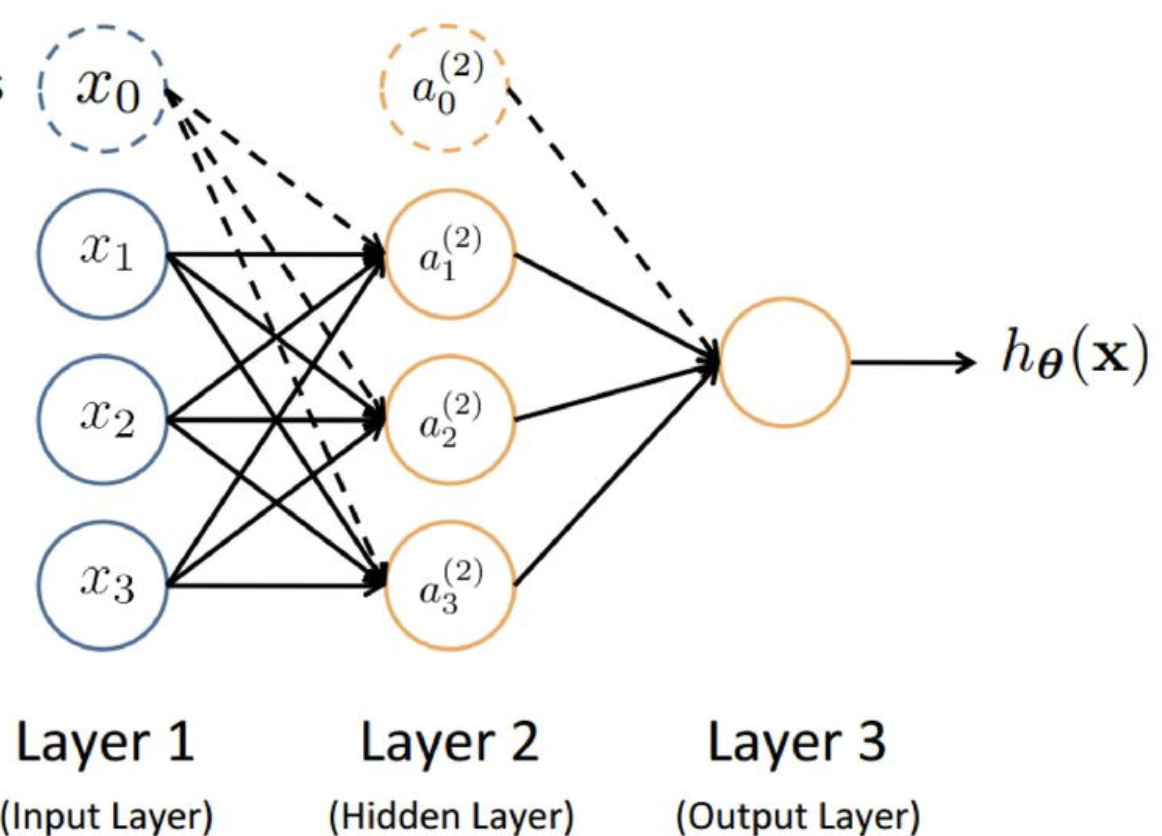
\includegraphics[width=0.78\textwidth]{../assets/NeuralNets.png}
  \caption{A one-hidden-layer feedforward neural network.  The supplied course
  illustration is based on Andrew Ng's teaching materials.}
  \label{fig:nn-schematic}
\end{figure}

Each circle is a \emph{unit} or \emph{neuron}.  Add a constant input $x_0=1$.
For hidden unit $j\in\{1,2,3\}$, define
\begin{equation}
  a_j^{(2)}=
  f^{(1)}\!\left(\theta_{0j}^{(1)}+
             \sum_{k=1}^3\theta_{kj}^{(1)}x_k\right),
  \label{eq:nn-hidden-unit}
\end{equation}
where the weighted sum is the input to the unit and $f^{(1)}$ is its activation
function.  The output is
\begin{equation}
  h_\theta(x)=
  f^{(2)}\!\left(\theta_0^{(2)}+
             \sum_{j=1}^3\theta_j^{(2)}a_j^{(2)}\right).
  \label{eq:nn-output}
\end{equation}
The network in Figure~\ref{fig:nn-schematic} has
$(3+1)\times3+(3+1)\times1=16$ weights and intercepts.

A familiar activation is the logistic, or sigmoid, function
\begin{equation}
  \sigma(z)=\frac{1}{1+e^{-z}}.
  \label{eq:nn-sigmoid}
\end{equation}
Other common choices include the rectified linear unit
$\max\{0,z\}$ and hyperbolic tangent.  For a continuous outcome, the output
activation is often the identity; for a binary probability, a sigmoid output
is natural.

\begin{example}[Approximating a binary maximum]
Let $x_1,x_2\in\{0,1\}$ and $h(x)=\max\{x_1,x_2\}$.  The single sigmoid unit
\[
  h_\theta(x)=\sigma(-20+40x_1+40x_2)
\]
is already an excellent approximation:
\begin{align*}
  h_\theta(0,0)&=\sigma(-20)\approx0,\\
  h_\theta(1,0)=h_\theta(0,1)&=\sigma(20)\approx1,\\
  h_\theta(1,1)&=\sigma(60)\approx1.
\end{align*}
The original notes used inconsistent coefficient subscripts; the expression
above uses the intercept and the two input coefficients explicitly.
\end{example}

Networks can be generalized in several directions:
\begin{itemize}
  \item a hidden layer can contain many more units than the input dimension;
  \item several hidden layers can be stacked to form a deep network;
  \item the output can be a vector, as in multiclass prediction; and
  \item inputs can include images or text after they are numerically encoded.
\end{itemize}
Universal-approximation results show that, under suitable activation and
regularity conditions, a one-hidden-layer network with sufficiently many units
can approximate a continuous function on a compact set arbitrarily well.  This
is an approximation result, not a promise that finite data and an optimization
algorithm will automatically find the best network.

For a visual experiment with architecture, activation functions, and training,
see \url{https://playground.tensorflow.org}.

\section{Conditional expectations as best predictors}
\label{sec:nn-best-predictor}

The key link with econometrics is a projection identity.  Suppose
$\E[Y^2]<\infty$.  Among all square-integrable measurable functions of $W$,
the conditional expectation minimizes mean squared error:
\begin{equation}
  m(W)=\E[Y\mid W]
  \in\arg\min_f\E[(Y-f(W))^2].
  \label{eq:nn-projection}
\end{equation}

\begin{proof}
Add and subtract $m(W)$ and expand:
\begin{align*}
  \E[(Y-f(W))^2]
  ={}&\E[(Y-m(W))^2]+\E[(m(W)-f(W))^2]\\
     &+2\E[(Y-m(W))(m(W)-f(W))].
\end{align*}
The cross term is zero because iterated expectations give
\begin{align*}
  &\E[(Y-m(W))(m(W)-f(W))]\\
  &\quad=\E\!\left[(m(W)-f(W))
        \E[Y-m(W)\mid W]\right]=0.
\end{align*}
The first term does not depend on $f$, and the second is nonnegative.  It is
minimized by $f(W)=m(W)$ almost surely.
\end{proof}

For treatment status $D\in\{0,1\}$, define
\begin{equation}
  m_d(w)=\E[Y\mid D=d,W=w].
  \label{eq:nn-treatment-regression}
\end{equation}
The corresponding population optimization problem is
\begin{equation}
  m_d(\cdot)\in
  \arg\min_h\E[(Y-h(W))^2\mid D=d].
  \label{eq:nn-population-loss}
\end{equation}
The argument of the minimum is a \emph{function}; it is not the numerical
conditional mean evaluated at one unspecified $W$.

\section{From population loss to a trained network}

Approximate $m_d(w)$ by $h_{d;\theta}(w)$.  In the subsample with $D_i=d$,
empirical risk minimization chooses
\begin{equation}
  \widehat\theta_d\in
  \arg\min_\theta
  \frac{1}{n_d}\sum_{i:D_i=d}
  \bigl(Y_i-h_{d;\theta}(W_i)\bigr)^2,
  \qquad n_d=\sum_i\1\{D_i=d\},
  \label{eq:nn-erm}
\end{equation}
and the estimated conditional mean is
$\widehat m_d(w)=h_{d;\widehat\theta_d}(w)$.  A propensity score can be trained
similarly with a binary cross-entropy loss and sigmoid output.

In practice, the numerical optimizer updates weights by backpropagation and a
gradient-based method.  Architecture, regularization, learning rate, number of
epochs, and early stopping are tuning choices.  Predictive performance should
be assessed on validation data rather than on the same observations used to
fit a highly flexible model.

\subsection{Advantages}

\begin{itemize}
  \item Networks can model nonlinearities and interactions in high-dimensional
        $W$ without specifying each one by hand.
  \item Categorical, text, and image inputs can be handled after appropriate
        numerical encoding.
  \item Matrix operations can be accelerated substantially on GPUs for large
        problems.
\end{itemize}

\subsection{Limitations and inference}

\begin{itemize}
  \item Training is nonconvex and can be sensitive to scaling, architecture,
        initialization, and regularization.
  \item A highly accurate predictor need not extrapolate well or identify a
        causal parameter when the research design is invalid.
  \item Standard errors for every point of a flexible fitted CATE surface are
        not obtained by treating network weights like coefficients in a small
        linear regression.
\end{itemize}

Neural networks can nevertheless serve as nuisance estimators inside
cross-fitted doubly robust or double-machine-learning procedures.  If the
nuisance estimates satisfy suitable rate and regularity conditions, the final
low-dimensional ATE estimator can have valid asymptotic inference even though
the individual network weights have no simple inferential interpretation.

\section{Application: DeepIV}
\label{sec:nn-deepiv}

Hartford, Lewis, Leyton-Brown, and Taddy (2017) study sponsored-search position
effects.  An advertiser's position on a Bing search page is endogenous: latent
user intent affects both placement and the probability of a click.  Their
DeepIV approach uses flexible neural networks in a nonparametric instrumental-
variables procedure.

The instruments include indicators for randomized experiments in which
advertiser--query pairs were assigned to different scoring algorithms.  These
experiments generate variation in advertisement position.  Covariates include
high-dimensional information such as the search query, and the sample exceeds
20 million observations.  The empirical analysis finds, among other results,
that a favorable position is especially valuable to small websites for
on-brand queries.

The original implementation is available at
\url{https://github.com/jhartford/DeepIV}.  It is historically important, but
software ecosystems evolve; contemporary replication should pin package
versions and test the environment before class.

\section{A small R illustration}
\label{sec:nn-r}

The following code uses the lightweight \texttt{nnet} package to approximate a
nonlinear conditional mean.  It is deliberately small enough to run through
Quarto Live in a browser.

\begin{rcode}
library(nnet)

set.seed(5280)
n <- 700
W1 <- runif(n, -1, 1)
W2 <- runif(n, -1, 1)
m <- sin(pi * W1) + W2^2
Y <- m + rnorm(n, sd = 0.25)

train <- sample(seq_len(n), 500)
dat <- data.frame(Y, W1, W2)

fit_nn <- nnet(Y ~ W1 + W2, data = dat[train, ],
               size = 8, linout = TRUE,
               decay = 0.01, maxit = 500, trace = FALSE)
fit_lm <- lm(Y ~ W1 + W2, data = dat[train, ])

test <- setdiff(seq_len(n), train)
pred_nn <- predict(fit_nn, dat[test, ])
pred_lm <- predict(fit_lm, dat[test, ])

c(neural_net = mean((Y[test] - pred_nn)^2),
  linear_model = mean((Y[test] - pred_lm)^2))
\end{rcode}

This comparison is about prediction, not causal identification.  It shows only
that a nonlinear architecture can approximate a nonlinear regression function
more flexibly than a misspecified additive linear model.

\section*{Summary}

\begin{itemize}
  \item A neural network composes weighted sums and activation functions to
        form a flexible global approximation.
  \item The conditional expectation is the population squared-error minimizer,
        which connects prediction to causal nuisance functions.
  \item Training replaces the population loss by an empirical loss and requires
        tuning, regularization, and honest validation.
  \item Neural networks do not create causal identification, but they can be
        useful nuisance estimators inside valid causal designs and cross-fitted
        doubly robust procedures.
\end{itemize}
